\chapter{Related Work}

\section{Code-Size Optimisations}

Although initially motivated by performance, many of the classical optimisations achieve better performance by reducing code size.
A small code, besides having fewer instructions to execute, can also have a positive impact on the cache utilisation.
Classical optimisations that are effective in reducing code size include the elimination of redundant, unreachable, and dead code, as well as certain kinds of strength reduction~\cite{cocke70,briggs97,debray00}.
In this section, we will describe some of these classical size-reducing optimisations.

\subsection{Constant Folding}

Constant folding is an optimisation that operates on the instruction level, identifying instructions whose operands are constant values, performing the evaluation of the instruction at compile time, and replacing it by the resulting value.
The effectiveness of constant folding can be augmented by combining it with constant propagation.
Constant folding reduces code size by eliminating instructions that can be computed at compile time.
Moreover, constant folding also works as an enabler to other optimisations, such as unreachable-code elimination (Section~\ref{sec:relatedwork:unreachable}).
 
\subsection{Unreachable-Code Elimination} \label{sec:relatedwork:unreachable}

Some functions may contain code that is unreachable. A code is unreachable if there is no valid control-flow path from the function's entry point that leads to it.
Since unreachable code is guaranteed to never be executed, compilers should remove it to avoid code bloat.

Often, unreachable code is uncovered by other optimisations.
For example, after constant propagation and constant folding, a conditional branch could have its condition evaluating to a constant, eliminating a path to one of its successor basic block.
If no other path leads to that basic block, it becomes unreachable.

The algorithm to eliminate unreachable code works in a mark-sweep manner, performing two passes over the basic blocks of the CFG.
The reachability analysis optimistically assumes that all basic blocks are dead until proven otherwise.
First, it marks all blocks as unreachable.
Next, starting from the entry point, it marks each block that it can reach as reachable.
If all branches and jumps are unambiguous, then all unmarked blocks can be deleted.
With ambiguous branches or jumps, the compiler must preserve any block that the branch or jump can reach.
This analysis is simple and inexpensive.

\subsection{Dead-Code Elimination}

A value definition is dead if it is not used on any path from the point in which it is defined to the exit point of the function.
In a similar way, an instruction is dead if it computes only values that are not used on any execution path leading from the instruction.
Any dead definition or instruction can be simply removed without altering the program's semantics, therefore reducing code size~\cite{muchnick98}.

The algorithm to eliminate dead code has some similarities with that for unreachable-code elimination described in Section~\ref{sec:relatedwork:unreachable}.
This algorithm also works in a mark-sweep manner~\cite{cooper07}.
First, the algorithm marks \textit{critical} instructions as \textit{alive}.
An instruction is \textit{critical} if it has an observable effect, for example, if it is a return instruction, a branch instruction, a function call, a memory operation, any instruction with side effect, etc.
Then, the algorithm follows the \textit{use-def chain} of every alive instruction, marking the operand instructions as alive.
This process continues until no more instructions can be marked as alive.
Finally, the sweep phase removes all instructions that have not been marked as alive, reducing code size.

\section{Merging Identical Functions}

In this section, we will discuss existing optimisations for merging identical functions.
Figure~\ref{fig:example-identical} illustrates how identical functions can appear in real programs.
The first pair of functions, shown in Figure~\ref{fig:example-identical-1-sphinx3}, were extracted from the \texttt{482.sphinx3} benchmark.
The only difference between these two functions is in their parameter type.
However, all pointer types can be considered equivalent since they can be bitcasted in a losslessly way.
These functions are usually produced by copy-and-paste programming, where a given code pattern is copied and then repurposed~\cite{kim04,jablonski10,ahmed15}.
The second pair of functions, shown in Figure~\ref{fig:example-identical-2-gcc}, were extracted from the \texttt{403.gcc} benchmark and they are fully identical.
These functions are part of GCC's backend, where it is common to have code that is automatically generated from a machine description~\cite{muchnick98,kolek13,ghica15}.

\begin{figure}[h]
\centering
\begin{subfigure}{\textwidth}
\centering
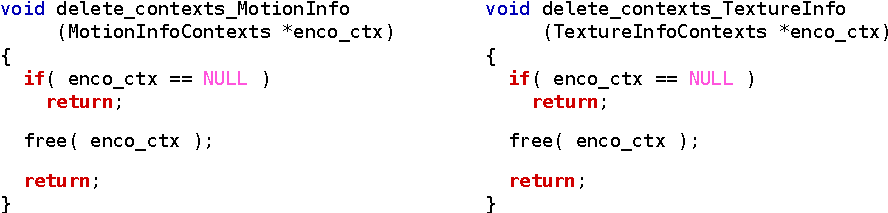
\includegraphics[scale=0.9]{src/relatedwork/figs/example-identical-1-sphinx3}
\caption{Two semantically identical functions extracted from the \texttt{482.sphinx3} benchmark.}
\label{fig:example-identical-1-sphinx3}
\end{subfigure}
\begin{subfigure}{\textwidth}
\centering
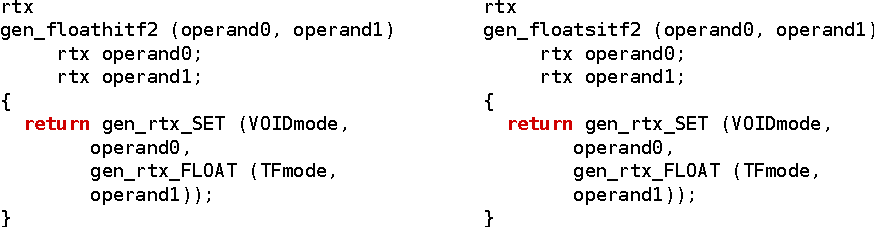
\includegraphics[scale=0.9]{src/relatedwork/figs/example-identical-2-gcc}
\caption{Two semantically identical functions extracted from the \texttt{403.gcc} benchmark.}
\label{fig:example-identical-2-gcc}
\end{subfigure}
\caption{Example of identical functions.}
\label{fig:example-identical}
\end{figure}

\begin{figure}[h]
\centering
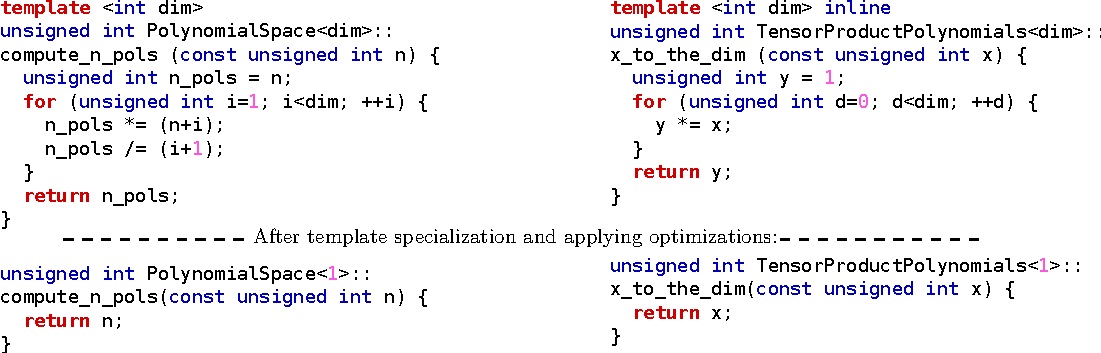
\includegraphics[scale=0.9]{src/relatedwork/figs/identical-example}
\caption{Two function extracted from the \texttt{447.dealII} benchmark that are not identical at the source level, but after applying template specialisation and optimisations they become identical at the IR level.}
\label{fig:identical-example}
\end{figure}

Note, however, that functions can be identical at the IR or machine level without necessarily being identical at the source level.
Figure~\ref{fig:identical-example} shows two real functions extract from the
447.dealII program in the SPEC CPU2006~\cite{spec} benchmark suite.
Although these two functions are not identical at the source level, they become
identical after a template specialisation and some optimisations are applied, in
particular, constant propagation, constant folding, and dead-code elimination. 
Specialising \verb|dim| to $1$ enables to completely remove the loop in the
function \verb|PolynomialSpace|.
Similarly, specializing \verb|dim| to $1$ results in only the first iteration
of the loop in the function \verb|TensorProductPolynomials| being executed.
The compiler is able to statically analyze and simplify the loops in both
functions, resulting in the identical functions shown at the bottom of
Figure~\ref{fig:identical-example}.

Identical code is particularly common in C++ programs
with heavy use of \textit{parametric polymorphism}, via template or \textit{auto} type deduction.



\section{Merging Identical Object Code}

The simplest way of merging identical functions is by looking at their object code, during link time.
\textit{Identical code folding}~(ICF) is an optimisation that identifies and merges two or more read-only sections, typically functions, that have identical contents.
This optimisation is commonly found in major linkers, such as \textit{gold}~\cite{tallam10,kwan12}, LLVM's \textit{lld}, and the MSVC linker~\cite{msvc-icf}.

Figure~\ref{fig:icf-example} shows an example, adapted from Tallam~\etal~\cite{tallam10},
of how generic programming in C++ can lead to identical functions in the object file.
The C++ code in in Figure~\ref{fig:icf-example-code} presents
a simple \textit{template class} and its member function being
instantiated multiple times with different pointer types.
Figure~\ref{fig:icf-example-object} shows the object code 
targeting the Intel x86 architecture.
For each instantiation of \textit{Foo}, a replica of its member
function \textit{getElement} is created.
Because the size of the different pointer types is the same,
all replicas of \textit{getElement} are identical
in the object file, which can be easily confirmed by
comparing their binary representation. as shown in
Figure~\ref{fig:icf-example-object}.

\begin{figure}[h]
% \begin{tabular}{cc}
% \begin{subfigure}{.5\textwidth}
% \begin{minted}[
% frame=lines,
% framesep=2mm,
% baselinestretch=1,
% %bgcolor=LightGray,
% fontsize=\footnotesize,
% %linenos
% ]{c++}
% template<typename T>
% class Foo {
%   ...
%   T element;
% public:
%   ...
%   T getElement() {
%     return element;
%   }
% };

% int main() {
%   Foo<int *> p;
%   Foo<float *> q;
%   Foo<void *> r;
%   ...
%   auto *pptr = p.getElement();
%   auto *qptr = q.getElement();
%   auto *rptr = r.getElement();
%   ...
% }
% \end{minted}
% \caption{A \textit{template class} with several instantiations.}
% \label{fig:icf-example-code}
% \end{subfigure} &
% \begin{subfigure}{.5\textwidth}
% \vspace{10ex}
% \begin{minted}[
% escapeinside=||,
% %fontfamily=tt,
% frame=lines,
% framesep=2mm,
% baselinestretch=1,
% %bgcolor=LightGray,
% fontsize=\scriptsize,
% %linenos
% ]{nasm}
% ; Disassembly of Foo<int *>::getElement()
% section .text._ZN3FooIPiE10getElementEv:
% _ZN3FooIPiE10getElementEv:   ; Hex Code
%   mov  rax,QWORD PTR [rdi]  ; 48 8b 07
%   ret                        ; c3

% ; Disassembly of Foo<float *>::getElement()
% section .text._ZN3FooIPfE10getElementEv:
% _ZN3FooIPfE10getElementEv:   ; Hex Code
%   mov  rax,QWORD PTR [rdi]  ; 48 8b 07
%   ret                        ; c3

% ; Disassembly of Foo<void *>::getElement()
% section .text._ZN3FooIPvE10getElementEv:
% _ZN3FooIPvE10getElementEv:   ; Hex Code
%   mov  rax,QWORD PTR [rdi]  ; 48 8b 07
%   ret                        ; c3
% \end{minted}
% \vspace{7ex}
% \caption{Disassembled object file.}
% \label{fig:icf-example-object}
% \end{subfigure}
% \end{tabular}
\caption{Example showing how a member function of a \textit{template class}
  can produce code replication susceptible to \textit{identical code folding}.
  For each instantiation of \textit{Foo}, a replica of the function
  \textit{getElement} is created for the template instance.
  When instantiated with pointer types, the object code of these functions will be identical.}
\label{fig:icf-example}
\end{figure}

Most object file formats, such as the \textit{Executable and Linkable Format} (ELF)~\cite{tallam10,kwan12}, are structured as separate sections of content, each section containing a certain type of content.
The main types are code segment, different types of data segment, and relocation information.
Relocation information describes how to modify other sections, connecting symbolic references to their definition.
In other words, it assigns actual addresses for position-dependent code and data.
For example, when a program calls a function, the associated call instruction must transfer control to the proper destination address at execution.

It is common practice for linkers to place functions in separate sections, as exemplified in Figure~\ref{fig:icf-example-object}.
Therefore, merging identical functions can be generalised to the problem of merging identical sections.
Two sections are considered identical if they have the identical section flags, data, code, and relocations.
Two relocations are considered the identical if they have the same relocation types, values, and if they point to the same or identical sections.

Since this equality has a cyclic definition, ICF is defined as a fixed-point computation, i.e., it is applied repeatedly until a convergence is obtained.
There are two approaches with distinct trade-offs.
$(i)$ The pessimistic apprach starts with all sections marked as being different and then repeatedly compare them trying to prove their equality, grouping those found to be identical, including their relocations.
This approach is implemented in the widely used \textit{gold} linker.
$(ii)$ The optimistic apprach starts with all functions marked as potentially identical and then repeatedly compare trying to disprove their equality, partitioning those found to be different.
This approach is implemented in LLVM's linker, \textit{lld}.

% \subsection{The Pessimistic Algorithm}

% The pessimistic algorithm is implemented in the gold linker.

% We can start with marking all functions as different and repeatedly do
% the checksumming.  This has the advantage that we do not need to wait
% for convergence. We can stop at any point and correctness will be
% guaranteed although not all cases would have been found.  However, this
% has a problem that some cases can never be found even if it is run until
% convergence.  Here is an example with mutually recursive functions :

% int funcA (int a)            int funcB (int a)
% {                            {
%   if (a == 1)                  if (a == 1)
%     return 1;                    return 1;
%    return 1 + funcB(a - 1);     return 1 + funcA(a - 1);
% }                            }

% In this example funcA and funcB are identical and one of them could be
% folded into the other.  However, if we start with assuming that funcA
% and funcB are not identical, the algorithm, even after it is run to
% convergence, cannot detect that they are identical.


% \subsection{The Optimistic Algorithm}

% The optimistic algorithm is implemented in LLVM linker, lld.

\begin{figure}[h]
% \begin{tabular}{cc}
% \begin{subfigure}{.5\textwidth}
% \begin{minted}[
% frame=lines,
% framesep=2mm,
% baselinestretch=1,
% %bgcolor=LightGray,
% fontsize=\footnotesize,
% %linenos
% ]{c++}
% int zip() {
%   return 0;
% }
% int zap() {
%   return 0;
% }
% int foo() {
%   return zip ();
% }
% int bar() {
%   return zap ();
% }
% \end{minted}
% \caption{A \textit{template class} with several instantiations.}
% \label{fig:icf-example-code}
% \end{subfigure} &
% \begin{subfigure}{.5\textwidth}
% \begin{minted}[
% escapeinside=||,
% frame=lines,
% framesep=2mm,
% baselinestretch=1,
% %bgcolor=LightGray,
% fontsize=\scriptsize,
% %linenos
% ]{gas}

% section .text._Z3zipv:
% _Z3zipv:                 ; Hex Code
%  xor eax, eax            ; 31 c0
%  ret                     ; c3    

% section .text._Z3zapv:
% _Z3zapv:
%  xor eax, eax            ; 31 c0
%  ret                     ; c3

% section .text._Z3foov:
% _Z3foov:
%  push rax                ; 50
%  call   6 |<\_Z3foov+0x6>|  ; e8 00 00 00 00
%  pop rcx                 ; 59
%  ret                     ; c3
% section .rela.text._Z3foov ; Relocation
% ; Type         Addend  Name
%  X86_64_PC32    -4      _Z3zipv

% section .text._Z3barv:
% _Z3barv:
%  push rax                ; 50
%  call   6 |<\_Z3barv+0x6>|  ; e8 00 00 00 00
%  pop rcx                 ; 59
%  ret                     ; c3
% section .rela.text._Z3barv ; Relocation
% ; Type         Addend  Name
%  X86_64_PC32    -4      _Z3zapv

% \end{minted}
% \caption{Disassembled object file.}
% \label{fig:icf-example-object}
% \end{subfigure}
% \end{tabular}
\begin{subfigure}{\textwidth}
\centering
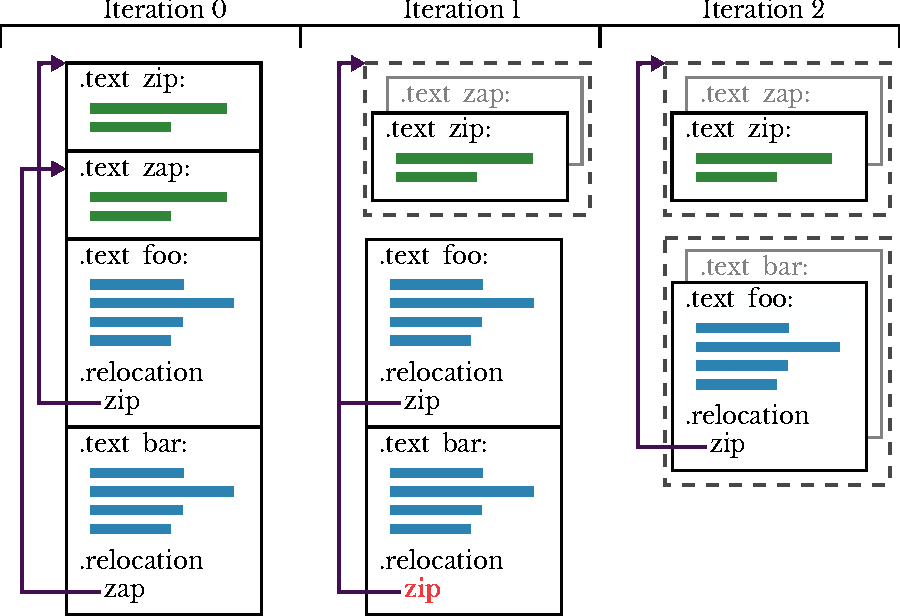
\includegraphics[width=0.9\textwidth]{src/relatedwork/figs/icf-example}
\caption{.}
\label{fig:identical-example}
\end{subfigure}

\caption{Example showing how a member function of a \textit{template class}
  can produce code replication susceptible to \textit{identical code folding}.
  For each instantiation of \textit{Foo}, a replica of the function
  \textit{getElement} is created for the template instance.
  When instantiated with pointer types, the object code of these functions will be identical.}
\label{fig:icf-example}
\end{figure}


\subsection{Identical Function Merging}

A similar optimisation for merging identical functions, but instead at the
intermediate representation (IR) level, is also offered by both GCC and
LLVM~\cite{llvm-fm,livska14}.
%The function merging optimisation currently offered by LLVM is only able to
%merge identical functions.
This optimisation is only flexible enough to accommodate simple type mismatches
provided they can be bitcasted in a losslessly way.

%%%%%%%%%%%%%%%%%%%%%%%%%%%%%%%%%%%%%%%%%%%%%%%%%%%%%%%%%%%%%%%%%%%%%%%%%%%%%%%%

A very strict function comparator is used to identify if two functions are 
semantically equivalent.
First it compares the signature and other general attributes of the two functions.
The functions must have identical signature, i.e., the same return type, the same
number of arguments, and exactly the same list of argument types.
Then this function comparator performs a simultaneous walk, in depth
first order, in the functions' control-flow graphs.
This walk starts at the entry block for both functions, then takes each block
from each terminator in order.
As an artifact, this also means that unreachable blocks are ignored.
Finally, it iterates through each instruction in each basic block.
Two blocks are equivalent if they have equivalent instructions in exactly the
same order, without excess.
The comparator always fails conservatively, erring on the side of claiming that
two functions are different.

When a pair of equivalent functions is identified, we can create either
an alias or a \textit{thunk}.
Aliasing etails eliminating one of the functions and replacing all its callsites
to the other function.
Thunks must be created when neither of the equivalent functions can be eliminated
by aliasing.
In such case, a thunk is created for either one of the functions, replacing its
body by a call to the other function, which allows all callsites and name
references to both functions to be preserved.
%In such case, the body of one of the functions is replaced by a call to the
%other function, and all callsites to both functions are preserved.
Aliasing is prefered since it is cheaper and adds no runtime overhead.
The appropriate merging is applied according to following rules:
\begin{itemize}
\item If the address of at least one function is not taken, alias can be used.
\item But if the function is part of COMDAT section that can be replaced, we
must use thunk.
\item If we create a thunk and none of functions is writeable, we can redirect calls
instead.
\end{itemize}
%%%%%%%%%%%%%%%%%%%%%%%%%%%%%%%%%%%%%%%%%%%%%%%%%%%%%%%%%%%%%%%%%%%%%%%%%%%%%%%%
%Similarly to the technique proposed by Edler von Koch~et~al.~\cite{edler14},
%LLVM's optimisation also exploits structural similarity among functions.
%However, the current implementation does not allow instructions to differ in
%their opcodes or in the number and type of their input operands.
Although very restrictive, this optimisation guarantees that any pair of
mergeable functions will result in code size reduction with no performance
overhead.

%Its simplicity also benefits compilation time, as the actual merge operation
%is trivial.
Its simplicity also allows for an efficient exploration approach based on computing
a hash of the functions and then using a binary tree to identify equivalent
functions.
%%%%%%%%%%%%%%%%%%%%%%%%%%%%%%%%%%%%%%%%%%%%%%%%%%%%%%%%%%%%%%%%%%%%%%%%%%%%%%%%
%We define a congruent group as a set of functions that are candidates for
%function equality.
%To create congruent groups, we build a compound hash value for each previously
%parsed function.
%%%As an optimisation, a hash of the function structure is calculated first, and
%%%two functions are only compared if they have the same hash.
Since hashing is cheap to compute, it allows us to efficiently
%Hashing is used to
group possibly equivalent functions and filter out functions
that are obviously unique.
%This hash is cheap to compute,
This hash must have the property that if function $F = G$
according to the comparison function, then $hash(F) = hash(G)$.
Therefore, as an optimisation, two functions are only compared if they have the
same hash.
This consistency property is critical to ensuring all possible merging
opportunities are exploited.
Collisions in the hash affect the speed of the pass but not the correctness
or determinism of the resulting transformation.

A function hash is calculated by considering only the number of arguments and
whether a function is varargs, the order of basic blocks (given by the
successors of each basic block in depth first order), and the order of
opcodes of each instruction within each of these basic blocks.
This mirrors the strategy of compare() uses to compare functions by walking the BBs in depth
first order and comparing each instruction in sequence. Because this hash
does not look at the operands, it is insensitive to things such as the
target of calls and the constants used in the function, which makes it useful
when possibly merging functions which are the same modulo constants and call
targets.


All functions can be sorted based on their hash value, which ends up grouping
possibly equivalent functions together.
If the hash value of a given function matches any of its adjacent values in
the sorted list, this function must be considered for merging.
%After that, the pass sorts each function to a congruent class according to
%its hash value.
%All functions in the module, ordered by hash.
Functions with a unique hash value can be easily ignored since no other function
will be found equivalent.
%Functions with a unique hash value are also easily eliminated.
%Otherwise it is dropped and never considered again.


The functions that remain are inserted into a binary tree, where functions are
the node values themselves.
An order relation is defined over the set of functions.
We need total-ordering, so we need to maintain four properties on the functions set:
\begin{itemize}
\item $a <= a$ (reflexivity);
\item if $a <= b$ and $b <= a$ then $a = b$ (antisymmetry);
\item if $a <= b$ and $b <= c$ then $a <= c$ (transitivity);
\item for all $a$ and $b$, $a <= b$ or $b <= a$ (totality).
\end{itemize}
This total-ordering was made through special function comparison procedure that
returns:
\begin{itemize}
\item 0 when functions are semantically equal,
\item -1 when Left function is less than right function, and
\item 1 for opposite case.
\end{itemize}

Functions are kept on binary tree. For each new function F we perform
lookup in binary tree.

%After the previous step is finished, all candidates in a group must be proved to
%be really semantically equivalent.

%Therefore, by construction, functions are hashed and grouped in O(n log n) time
%complexity.






\section{Merging Beyond Identical Functions}

In the previous sections, we have seen compiler optimisations that merge identical functions.
However, nearly identical functions, with only minor differences, are also commonly found.
Figure~\ref{fig:example-similar} shows two examples of nearly identical functions found in real programs.
The highlighted differences prevent these functions from being merged by the identical function merging techniques.
%These functions are usually produced by copy-and-paste programming,
%where a given code pattern is copied and then repurposed~\cite{kim04,jablonski10,ahmed15}.
The first pair of functions, shown in Figure~\ref{fig:example-similar-1-hmmer}, illustrates code that is usually produced by copy-and-paste programming,
where a given code pattern is copied and then repurposed~\cite{kim04,jablonski10,ahmed15}.
The second pair of functions, shown in Figure~\ref{fig:example-similar-3-gcc}, are produced by generative programming~\cite{czarnecki99,draheim04}, where their code was
automatically generated using a description language~\cite{ghica15}.

\begin{figure}[h]
\centering
\begin{subfigure}{\textwidth}
\centering
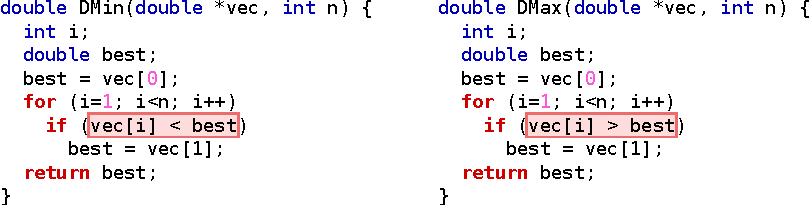
\includegraphics[width=0.9\textwidth]{src/relatedwork/figs/example-similar-1-hmmer}
\caption{Two similar functions extracted from the \texttt{456.hmmer} benchmark.}
\label{fig:example-similar-1-hmmer}
\end{subfigure}
%\begin{subfigure}{\textwidth}
%\centering
%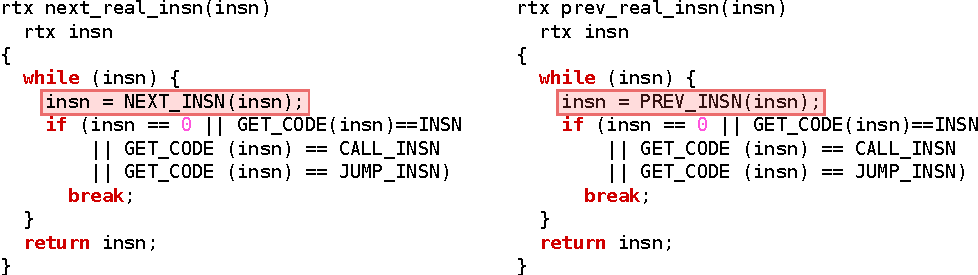
\includegraphics[width=0.9\textwidth]{src/relatedwork/figs/example-similar-2-gcc}
%\caption{Two similar functions extracted from the \texttt{403.gcc} benchmark.}
%\label{fig:example-similar-2-gcc}
%\end{subfigure}
\begin{subfigure}{\textwidth}
\centering
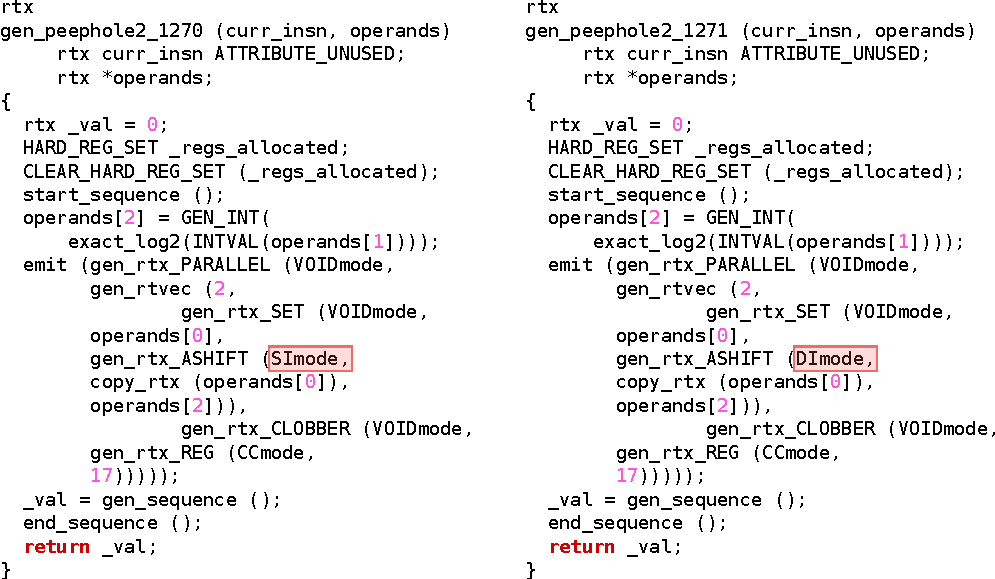
\includegraphics[width=\textwidth]{src/relatedwork/figs/example-similar-3-gcc}
\caption{Two similar functions extracted from the \texttt{403.gcc} benchmark.}
\label{fig:example-similar-3-gcc}
\end{subfigure}
\caption{Example of two pairs of highly similar functions. Because they are not identical, they cannot be merged by the function merging technique currently found in major compilers.}
\label{fig:example-similar}
\end{figure}


% The function merging technique presented in \cite{edler14} restricts merging to nearly identical functions.
% They only allow for pairs of corresponding instructions to differ if they still have equivalent data type.


Edler von Koch~et~al.~\cite{edler14} have proposed a function-merging technique which exploits structural similarity among functions.
Their optimization is able to merge nearly identical functions.
%similar functions that are not necessarily identical.
Two functions are structurally similar if both their function types are equivalent
and their CFGs are isomorphic.
Two function types are equivalent if they agree in the number, order, and types
of their parameters as well as
their return types, linkage type, and other compiler-specific properties.
In addition to the structural similarity of the functions, their technique also
requires that corresponding basic blocks have exactly the same number of instructions
and that corresponding instructions must have equivalent resulting types.
% but may differ in their opcodes or in the number and type of their input operands.
Mergeable functions are only allowed to differ in corresponding instructions,
where they can differ in their opcodes or in the number and type of their input operands.
Corresponding named values must have the same data type.
%The only differences that are actually allowed is that
%corresponding instructions can 
%differ in their opcodes or in the number and type of their input operands.


%If two corresponding instructions have different opcodes, they split the basic
%block and insert a switch branch to select which instruction to execute
%depending on a function identifier.

Because their technique is limited to functions with identical CFGs
and function types, once it merges a pair of functions, a third
\textit{similar} function cannot be merged into the resulting merged function
since they will differ in both CFGs and their lists of parameters.
Due to this limiting factor, the state-of-the-art has to first group
mergeable functions before simultaneously merging all functions within a group.

Their algorithm iterates simultaneously over corresponding basic
blocks in the set functions being merged, as they have isomorphic CFGs.
Figure~\ref{fig:soa-example-1} shows an example of two functions with isomorphic CFGs and their corresponding basic blocks arranged side by side.

\begin{figure}[h]
  \centering
  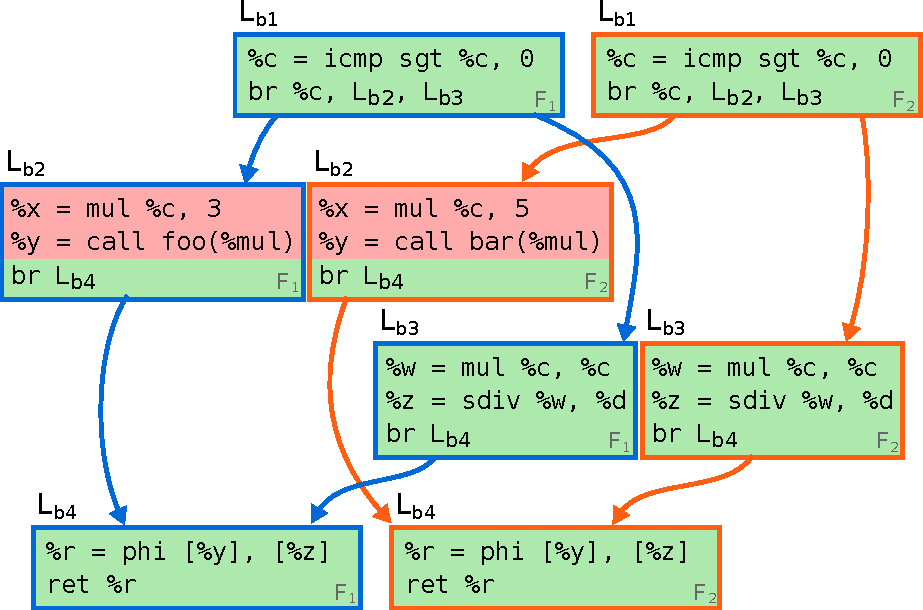
\includegraphics[width=0.8\textwidth]{src/relatedwork/figs/soa-example-1.pdf}
  \caption{An example of two functions with isomorphic CFGs and their corresponding basic blocks arranged side by side. Instructions in paired basic blocks are compared in a pairwise manner.}
  \label{fig:soa-example-1}
\end{figure}

Every pair of basic blocks have their instructions analysed in a pairwise manner.
Two instructions match if they have the same opcode with equivalent data types and operands.
Even if two instructions differ only on their operands, they are classified as mismatching.
For every pair of basic blocks, if their corresponding instructions have any difference, except for the data type of the computed value, the merged basic block is split by inserting a switch branch to select which instruction
to execute depending on a function identifier.
A phi-node is used to unify the mismatching instructions as a single named value.
This unification is only possible because they compute values of the equivalent data types.
Note that no operand selection is performed, every use of the mismatching instructions will refer to their phi-node.
Figure~\ref{fig:soa-example-2} shows an example of a merged basic block containing two mismatching pairs of instructions.
A split is added for every pair of mismatching instructions with the phi-node instruction added to the their immediate point of convergence.

% Because these instructions have equivalent resulting types, their results can be
% merged using a phi-operator, which can then be used transparently as operands
% by other instructions.

\begin{figure}[h]
  \centering
  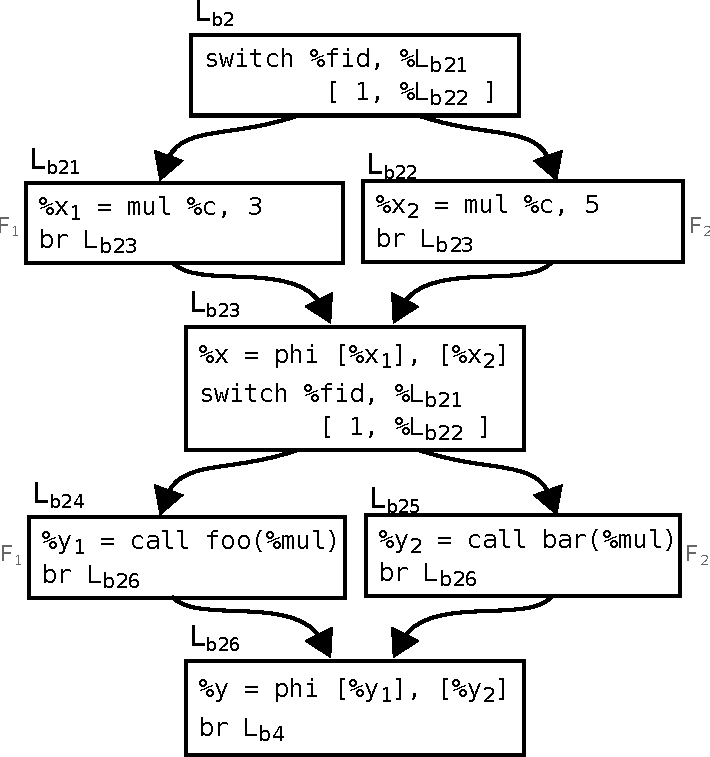
\includegraphics[width=0.6\textwidth]{src/relatedwork/figs/soa-example-2.pdf}
  \caption{An example of a merged basic block containing two mismatching pairs of instructions. A split is added for every pair of mismatching instructions with the phi-node instruction added to the their immediate point of convergence.}
  \label{fig:soa-example-2}
\end{figure}

Overall, except for mismatching pairs of instructions, the two functions must have identical function types, i.e., they must have the same return type and list of arguments, identical CFGs, with corresponding basic blocks having the same number of instructions.
Although this technique improves over LLVM's identical function merging, it is
still unnecessarily limited.
In Section~\ref{sec:motivation}, we showed examples of very similar real functions where the technique proposed by Edler von Koch~et~al.~\cite{edler14} fails to merge.
In Chapter~\ref{chp:cgo19} we introduce a novel technique that addresses such limitations improving on their technique across the board.

%%%%%%%%%%%%%%%%%%%%%%%%%%%%%%%%%%%%%%%%%%%%%%%%%%%%%%%%%%%%%%%%%%%%%%%%



\textbf{TODO: Comparison table: Identical vs VonKoch vs Ours}


\section{Code Factoring}

%Function merging and code factoring are different techniques for solving the
%same fundamental problem of duplicated code.
Code factoring refers to related techniques that address the same fundamental
problem of duplicated code in a different way.
%While the former works by merging similar functions, the latter works by
%factoring out duplicated code~\cite{loki04}.
%Instead of merging similar functions, code factoring works by factoring out
%duplicated code into separate functions~\cite{loki04}.
Code factoring can be applied at different levels of the program~\cite{loki04}.
Local factoring, also known as local code motion, moves identical instructions
from multiple basic blocks to either their common predecessor or successor,
whenever valid~\cite{knoop94,briggs94,loki04}.
Procedural abstraction %(or outlining)
finds identical code
that can be extracted into a separate function, replacing all replicated
occurrences with a function call~\cite{loki04,dreweke07}.

Procedural abstraction differs from function merging as it usually works on
single basic blocks or single-entry single-exit regions.
Moreover, it only works for identical segments of code, and every identical
segment of code is extracted into a separate new function.
Function merging, on the other hand, works on whole functions, which can be
identical or just partially similar, producing a single merged function.

However, all these techniques are orthogonal to the proposed optimization and
could complement each other at different stages of the compilation pipeline.




\section{Code Similarity}

Code similarity has also been used in other compiler optimizations or tools for
software development and maintenance.
In this section, we describe some of these applications.

Coutinho~et~al.~\cite{coutinho11} proposed an optimization that uses instruction
alignment to reduce divergent code for GPU.
They are able to fuse divergent branches that contain single basic blocks,
improving GPU utilization.
%reducing idle cores.

Similarly, analogous algorithms have also been suggested to identify the
differences between two programs, helping developers with source-code
management and maintenance~\cite{yang91,miller85}.
These techniques are applied in tools for source-code management, such as
the \textit{diff} command~\cite{miller85}.

Similar techniques have also been applied to code editors and IDEs~\cite{toomim04,sajnani16}.
For example,
SourcererCC~\cite{sajnani16} detects possible clones, at the source level, by
dividing the programs into a set of code blocks where each code block is itself
represented by a bag-of-tokens, i.e., a set of tokens and their frequencies.
Tokens are keywords, literals, and identifiers, but not operators.
Code blocks are considered clones if their degree of similarity is higher than
a given threshold.
In order to reduce the number of blocks compared, candidate blocks are filtered
based on a few of their tokens where at least one must match.

Our ranking mechanism uses an approach similar to SourcererCC, where we use
opcode frequencies and type frequencies to determine if two functions are
likely to have similar code.
However, we need a precise and effective analysis of code similarity when
performing the actual merge.
To this end, we use a sequence alignment technique.



\section{Tuning Compilers with Deep Learning}

There is been many work using machine learning as a heuristic for tuning runtime systems~\cite{andreasson02,wang09,castro11,rocha17,pereira17} and compilers~\cite{cavazos05,leather09,cummins17,wang18,mendis19}.

Cavazos and O'Boyle~\cite{cavazos05} propose the use of genetic algorithm to tune the heuristics of function inlining.
They use genetic algorithm to optimise the values for different features that control the inlining heuristic.
%Some of these features are the size of the callee and caller functions.
These features are chosen by the compiler writer and they define the maximum size allowed by the inlining transformation for the callee and the caller functions, the maximum size for callee functions that are hot or that should always be inlined, etc.
The optimised features are then used to define the rules of the inlining heuristic, describing which call sites should be allowed for inlining.
The fitness function of the genetic algorithm involves the actual runtime of the compiled program, rendering the feature optimisation process very costly.
However, their approach is able to achieve significant speedups over the baseline.

The quality of these features is critical to the improvements resulting from machine learning solutions.
Leather~et~al.~\cite{leather09} propose the use of genetic programming in order to also automate the selection of these features.
The feature space is described by a grammar and is then searched with genetic programming and predictive modelling, to avoid recompilation of the program for each step in searching the optimization space.
The genetic programming technique is used to generate features that are fed to a decision tree.
This machine learning solution form the decision-making heuristics for the loop-unrolling optimisation.
They show that the automated selection of features outperform hand-coded features, for the same machine learning procedure based on decision trees.

Cummins~et~al.~\cite{cummins17} propose DeepTune, which uses deep neural networks to learn optimization heuristics directly on raw code, unifying the search for features and decision-making heuristics into a single learning model.
Since the program, in its textual form, can be seen as a sequence of tokens of variable length, using a recurrent neural networks becomes a natural choice.
DeepTune has an LSTM-based language model that processes raw code, producing a fixed-size encoding which is then fed to a heuristic model based on a feed-forward neural network.

Mendis~et~al.~\cite{mendis19} propose Ithemal, a tool which uses deep neural networks to predict the throughput of a set of machine instructions.
Ithemal can be used as a cost model for compiler optimisations and code generation, aiding the decision of whether a transformation would result in faster code.
Similar to DeepTune, Ithemal also processes raw machine instructions using an LSTM-based language model.
However, Ithemal has an architecture with two LSTM stages.
The first LSTM processes the tokens that compose one instruction.
The second LSTM processes the encoded instructions that are produced by the first LSTM.
The output of the second LSTM is aggregated into the final throughput prediction.